% !TeX encoding = UTF-8
% !TeX spellcheck = es_ES
% !TeX root = DccPowerDistribution.tex

Esta seccion es como empezar rapidamente con la configuracion por defecto, recomendamos leer todas las instrucciones para los diferentes
opciones de configuracion. 
\subsection{Soldaturas de los conectores}
El primer paso es escoger los conectores mas adecuados para nuestra maqueta, siendo la seccion de guia rapida, presuponemos que se utilizaran
los incluidos con el kit.

El segundo paso es soldar los conectores DCC, se suminstran unos JST XH 2.54, para dos y 4 vias. El de dos vias (J1) se usa para conectar a la señal DCC,
ya sea de la central o de un Booster. Mientras que J7, el conector de 4 vias, es la señal DCC
en TTL, valida para la libreria DCC de aurdino
\begin{figure}[h]
    \centering
    \begin{tikzpicture}
        \node[inner sep=0pt] (russell) at (0,0)
            {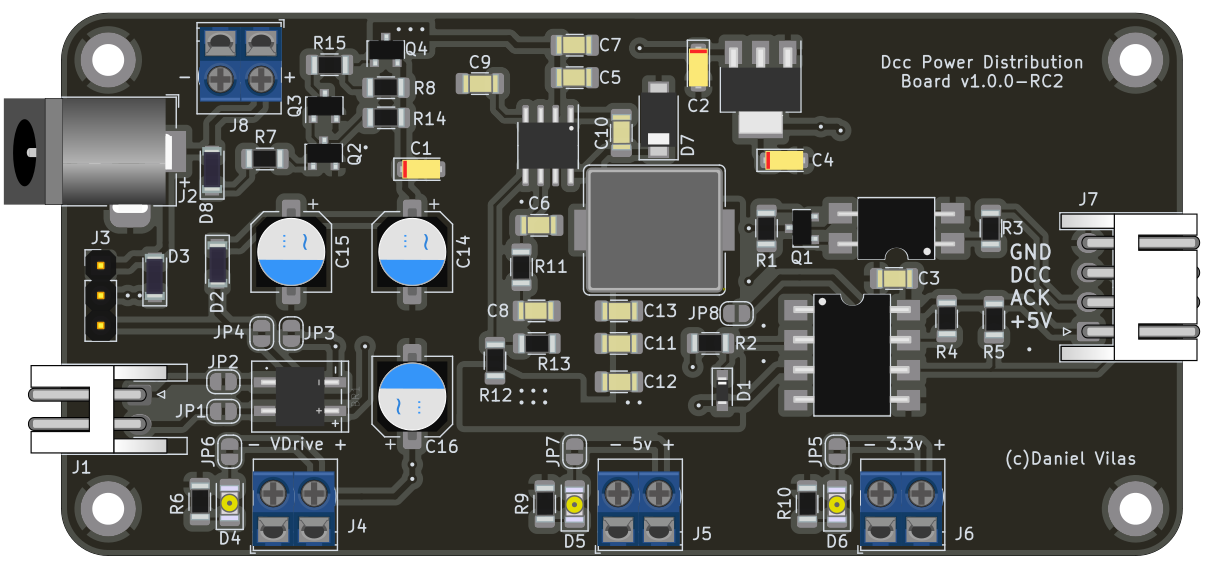
\includegraphics[scale=1.3]{images/front.png}};
        %\draw [very thin, green] (-6,-3) grid (6,3);
        \draw [color=red](-6.5,-0.7) rectangle (-4.5,-2.1); 
        \node [text width = 1cm] at (-7.1,-1.4){A la señal DCC};
        \draw [color=red](4.8,-1) rectangle (6.6,1.1);
        \node [text width = 1cm] at (7.2, 0.05){A un Decoder};
        %\node[below] {$a$};
    \end{tikzpicture}
    \caption{Conectores Dcc}
    \label{fig:DccConnectors}
\end{figure}

Los siguentes elementos a soldar, por tamaño, son los terminales para la salida de voltaje/corriente. 
En la guia rapida suponemos que se usan Los bloques terminales atornillables.

\begin{figure}[h]
    \centering
    \begin{tikzpicture}
        \begin{scope}
            \clip (-4.3,0) rectangle  (4.3,1.5);
            \node[inner sep=0pt] (russell) at (0.1,3)
                {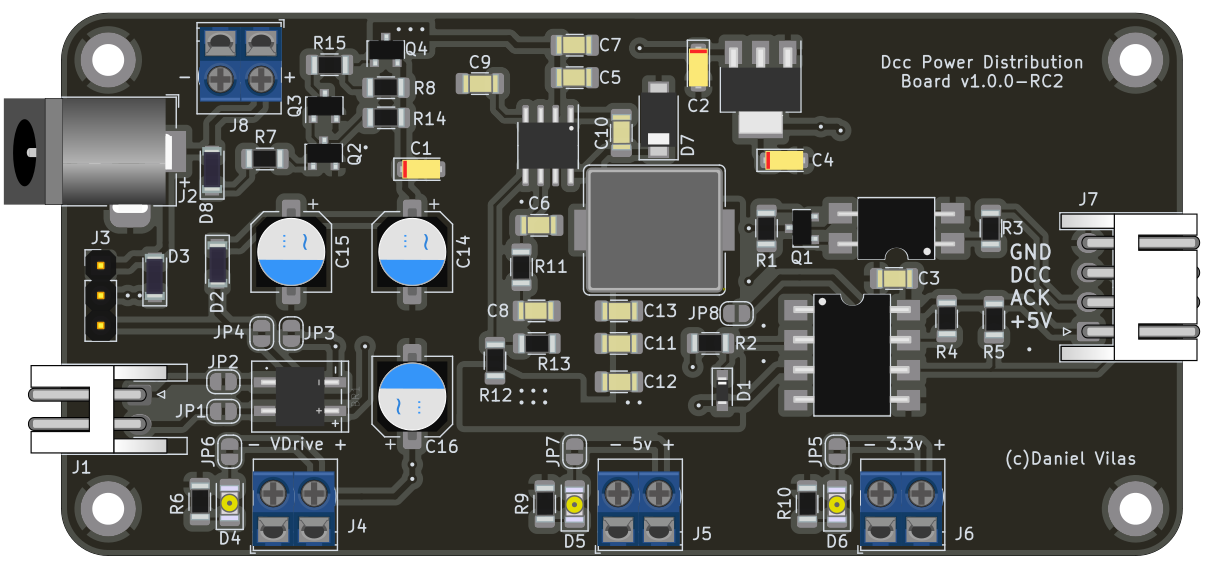
\includegraphics[scale=1.3]{images/front.png}};
        \end{scope}
        %\draw [very thin, green] (-5,-1) grid (5,2);
        \draw [color=red](-4,1.4) rectangle + (1.5,-1.6); 
        \node [text width = 1.3cm] at (-3.3,-0.5){VDrive};
        \draw [color=red](-0.2,1.4) rectangle + (1.5,-1.6); 
        \node [text width = 1.3cm] at (0.5,-0.5){+5V};
        \draw [color=red](2.7,1.4) rectangle + (1.5,-1.6); 
        \node [text width = 1.3cm] at (3.4,-0.5){+3.3V};
        %\node[below] {$a$};
    \end{tikzpicture}
    \caption{Salida Voltaje y Corriente}
    \label{fig:VccOutConnectors}
\end{figure}

Finalizaremos la soldadura añadiendo un solo conector de entrada, o bien el Jack o bien el terminal, segun lo que tengamos
disponible. Si vamos a usar un transformador con una jack (Centro positivo), soldaremos el Jack, pero si vamos a usar un
bus de corriente continua (dos cables) es mejor usar el terminal.

\begin{figure}[H]
    \centering
    \begin{minipage}{0.45\textwidth}
    \begin{tikzpicture}
        \centering
        \begin{scope}
            \clip (-2,-1.5) rectangle  +(4,2.9);
            %\draw [very thin, green, fill=yellow]  (-6,-3) rectangle (6,4);
            \node[inner sep=0pt] (russell) at (5,-1.9)
                {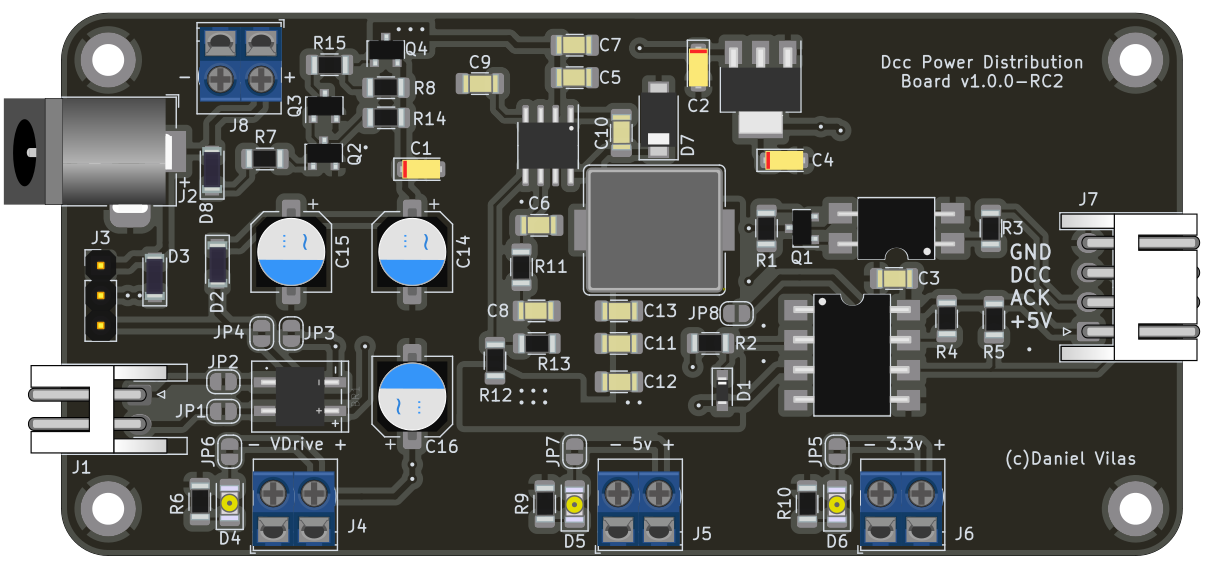
\includegraphics[scale=1.3]{images/front.png}};
            %\draw [very thin, green]  (-7,-3) grid (6,4);
        \end{scope}
        %\draw [very thin, green] (-3,-2) grid (3,2);
        \draw [color=red](-2,0.3) rectangle + (2.6,-1.6);
        \node [text width = 1.3cm] at (-2.5,-0.5){Jack 2mm};
    \end{tikzpicture}
    \caption{Entrada Voltaje Jack}
    \label{fig:VccInJack}
    \end{minipage}
    \hfill
    \begin{minipage}{0.45\textwidth}
    \centering
    \begin{tikzpicture}
        \begin{scope}
            \clip (-2,-1.5) rectangle  +(4,2.9);
            %\draw [very thin, green, fill=yellow]  (-6,-3) rectangle (6,4);
            \node[inner sep=0pt] (russell) at (5,-1.9)
                {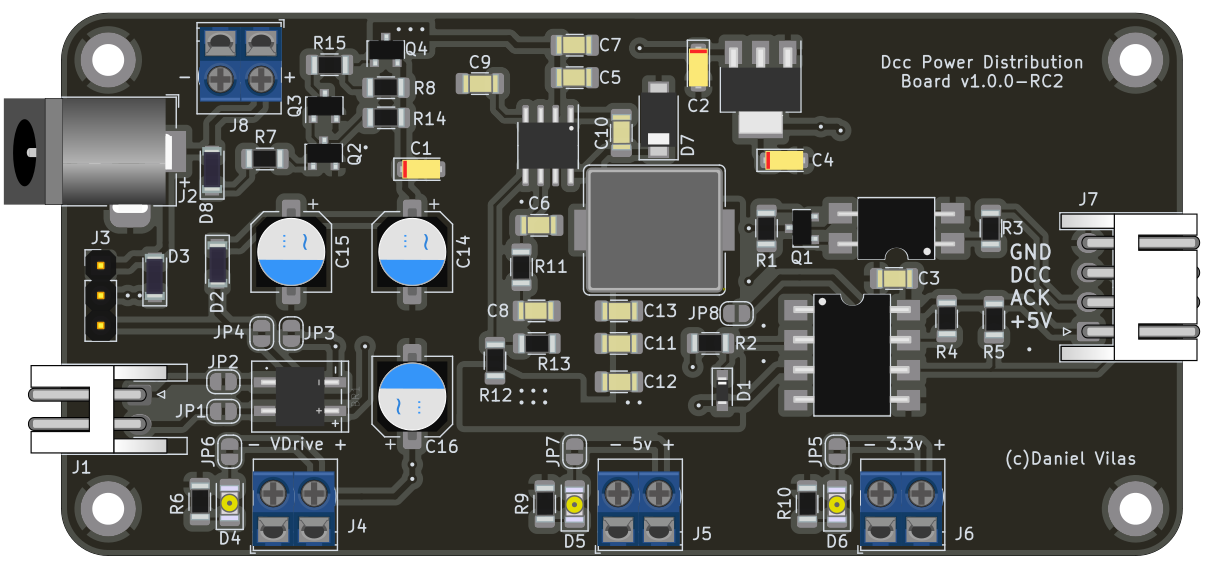
\includegraphics[scale=1.3]{images/front.png}};
            %\draw [very thin, green]  (-7,-3) grid (6,4);
        \end{scope}
        %\draw [very thin, green] (-3,-2) grid (3,2);
        \draw [color=red](0.2,-0.3) rectangle + (1.4,1.6);
        \node [text width = 1.3cm] at (1,2){Terminal Entrada};

    \end{tikzpicture}
    \caption{Entrada Voltaje Terminal}
    \label{fig:VccInTerminal}
    \end{minipage}
\end{figure}
Por ultimo como en cada proceso de soldadura, usar un tester para asegurarse antes de que no haya un cortocircuito
entre las soldaduras.
\subsection{Conexiones de entrada}
Con la maqueta apagada y el bus de alimentacion sin corriente, podremos procedera a conectar la entrada de alimentacion.
Tanto la señal DCC como la conexion a Corriente Continua. Para el conector DCC, hay que usar un cable terminado y 
crimpado con un Conector JST XH de dos vias, suministrado con el modulo, el otro exremo de este cable se debera conectar
a la central DCC o Booster como si fuera un tramo de via más.

\begin{figure}[H]
    \centering
    \begin{tikzpicture}
        \begin{scope}
            \clip (-1.5,-1) rectangle  + (3,2);
            %\draw [very thin, green, fill=yellow]  (-6,-3) rectangle (6,4);
            \node[inner sep=0pt] (russell) at (5.1,1.25)
                {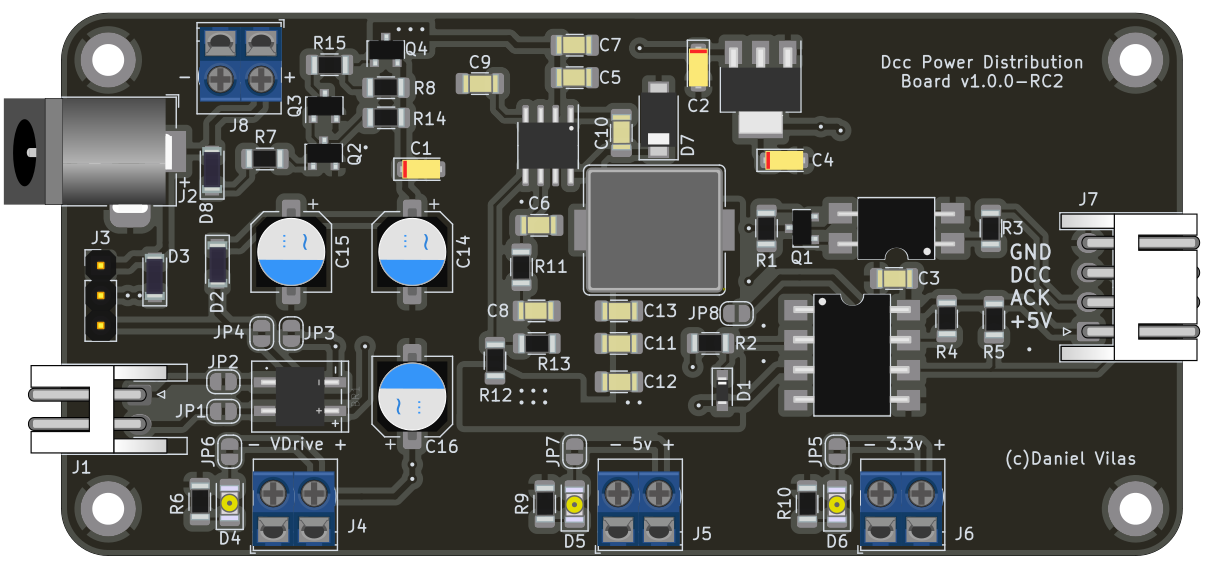
\includegraphics[scale=1.3]{images/front.png}};
            %\draw [very thin, green]  (-7,-3) grid (6,4);
        \end{scope}
        %\draw [very thin, green] (-3,-2) grid (3,2);
        \draw [color=red](-1.5,-0.9) rectangle + (2.3,1.5);
        \node [draw, text width = 2cm] at (-4,-0.15){Central o Booster};
        \draw [color=gray, line width=3pt,cap=round] (-2.9,0.06) -- (-1.4,0.06);
        \draw [color=lightgray, line width=3pt,cap=round] (-2.9,-0.25) -- (-1.4,-0.25);
    \end{tikzpicture}
    \caption{Entrada Señal DCC}
    \label{fig:DccIn}
\end{figure}
No es necesario una polaridad concreta, por lo que se pueden conectar a la via J o K indistintamente. No obstante se 
recomienda usar siempre la misma polaridad en todos los modulos iguales en la maqueta.

Si se va a usar un adaptador con un Jack 2mm, asegurarse de que sea centro positivo y conectarlo.
Pero en el caso de usar el terminal atornillable revisar la polaridad marcada en la placa con los simbolos + y -
\begin{figure}[H]
\centering
\begin{tikzpicture}
    \begin{scope}
        \clip (-1.5,-1) rectangle  +(3,2);
        %\draw [very thin, green, fill=yellow]  (-7,-3) rectangle (7,5);
        \node[inner sep=0pt] (russell) at (6.2,-3.55)
            {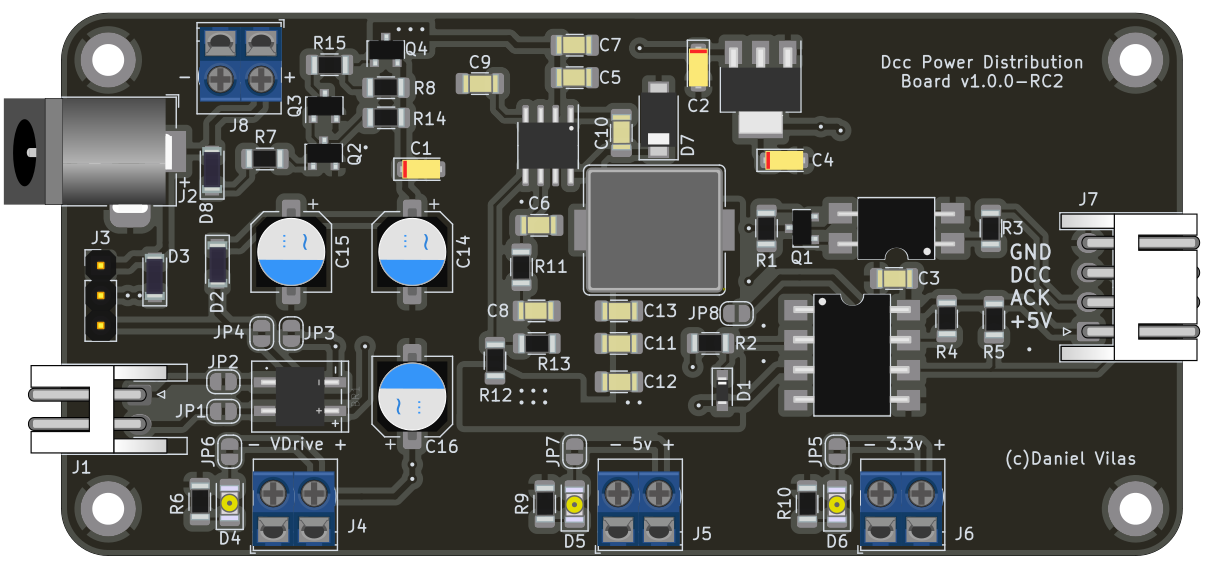
\includegraphics[scale=2]{images/front.png}};
        %\draw [very thin, green]  (-7,-3) grid (6,4);
    \end{scope}
    %\draw [very thin, green] (-3,-2) grid (3,2);
    \draw [color=red](-1.2,-0.8) rectangle + (2.2,2);
    \node [draw, text width = 1.7cm] at (-0.1,2.3){Adaptador CC};
    \draw [color=black, line width=3pt,cap=round] (-0.4,1.8) -- (-0.4,1.05);
    \draw [color=violet, line width=3pt,cap=round] (0.3,1.8) -- (0.3,1.05);
    \draw [color= yellow, line width=2pt] (-1,-0) circle[radius=0.3];
    \draw [color= yellow, line width=2pt] (.75,-0) circle[radius=0.3];
\end{tikzpicture}
\caption{Entrada Voltaje Terminal}
\label{fig:VccInTerminal2}
\end{figure}


Una vez conectado la alimentacion de entrada, podremos encender la maqueta y comprobar que todos los volajes
son correctos. Para ello se incluyen tres leds, uno para cada salida y se encenderan en cuanto haya voltaje
en dicha salida. Y ademas podremos medir con un polimetro
el voltaje entre los dos bornes del terminal.

\begin{figure}[h]
    \centering
    \begin{tikzpicture}
        \begin{scope}
            \clip (-4.3,0) rectangle  (4.3,1.5);
            \node[inner sep=0pt] (russell) at (0.1,3)
                {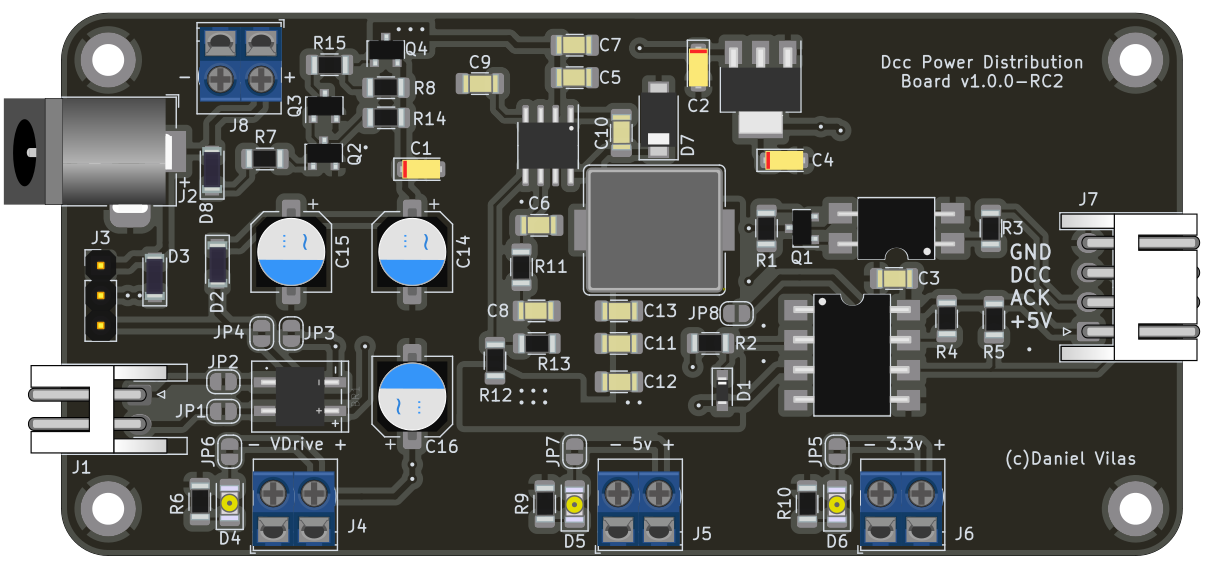
\includegraphics[scale=1.3]{images/front.png}};
        \end{scope}
        %\draw [very thin, green] (-5,-1) grid (5,2);
        \draw [color=red](-4,1.4) rectangle + (1.5,-1.6); 
        \node [text width = 1.3cm] at (-3.3,-0.5){VDrive};
        \draw [color=red](-0.2,1.4) rectangle + (1.5,-1.6); 
        \node [text width = 1.3cm] at (0.5,-0.5){+5V};
        \draw [color=red](2.7,1.4) rectangle + (1.5,-1.6); 
        \node [text width = 1.3cm] at (3.4,-0.5){+3.3V};
        \draw [color= yellow, line width=2pt] (-4.1,0.6) circle[radius=0.35];
        \draw [color= yellow, line width=2pt] (-0.3,0.6) circle[radius=0.35];
        \draw [color= yellow, line width=2pt] (2.6,0.6) circle[radius=0.35];
        %\node[below] {$a$};
    \end{tikzpicture}
    \caption{Salida Voltaje y Corriente}
    \label{fig:VccOutLeds}
\end{figure}

\subsection{Salida DCC}
Para conectar la alimentacion y las señales DCC a un Arduino, solo se necesita el conector JST XH de 4 vias. Para ello
se incluye un cable donde un estremo es JST XH y el otro son puntas macho Dupont sueltas. En la PCB esta marcado que señal
es cada cable.

\begin{figure}[H]
    \centering
    \begin{tikzpicture}
    \begin{scope}
        \clip (-2,-2) rectangle  + (4,4);
        %\draw [very thin, green, fill=yellow]  (-6,-4) rectangle (12,8);
        \node[inner sep=0pt] (russell) at (-8.1,0)
            {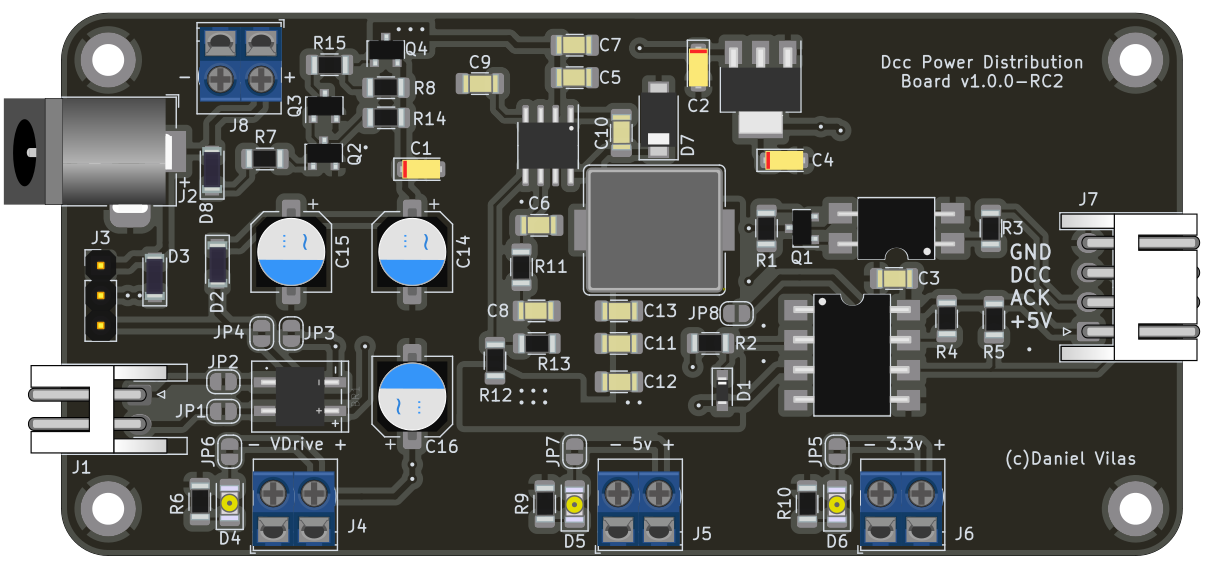
\includegraphics[scale=2]{images/front.png}};
        %\draw [very thin, green]  (-7,-3) grid (6,4);
    \end{scope}
    %\draw [very thin, green] (-3,-2) grid (3,2);
    \draw [color=yellow,line width=2pt](-1.6,-0.9) rectangle + (1.6,1.8);
    
    \node[right] at (4,1) {GND - A GND del aurdino};
    \node[right] at (4,0.33) {DCC - A Pin DCC (2)};
    \node[right] at (4,-0.33) {ACK - A Pin ACK (3)};
    \node[right] at (4,-1) {+5V - A 5V del Arduino)};
    
    \draw [color=black, line width=3pt,cap=round] (2.0,0.75) -- (4,1);
    \draw [color=blue, line width=3pt,cap=round] (2,0.25) -- (4,0.33);
    \draw [color=orange, line width=3pt,cap=round] (2,-0.25) -- (4,-0.33);
    \draw [color=red, line width=3pt,cap=round] (2.0,-0.75) -- (4,-1);
\end{tikzpicture}
    \caption{Entrada/Salida Señal DCC}
    \label{fig:DccOut}
\end{figure}
Por defecto la placa DCC Power Distribution esta configurada para que por la linea +5V
este conectada al bus de 5V de salida, por lo que se puede usar para alimentar un Arduino
sin problemas. Si el Arduino ya tiene su propia alimentacion, puede desconectarse este pin
o cambiar la configuracion de la placa. 

Los pines a los que conectar las señales DCC y ACK son 2 y 3 respectivamente para los
ejemplos de la libreria NmraDcc.

En este momento ya se puede encender la maqueta y usar el Arduino como decoder DCC.

\subsection{Otras salidas de Voltaje}
DCC Power Distribution incluye otras tres salidas de voltaje, a las que se pueden conectar
otros dispositivos, para ello solo hay que instalar los cables y respetar la polaridad
marcada con los simbolos + y -.

\begin{figure}[h]
    \centering
    \begin{tikzpicture}[scale=1]
        \begin{scope}
            \clip (-6.5,0) rectangle  +(13,2.5);
            \node[inner sep=0pt] (russell) at (0.1,4.75)
                {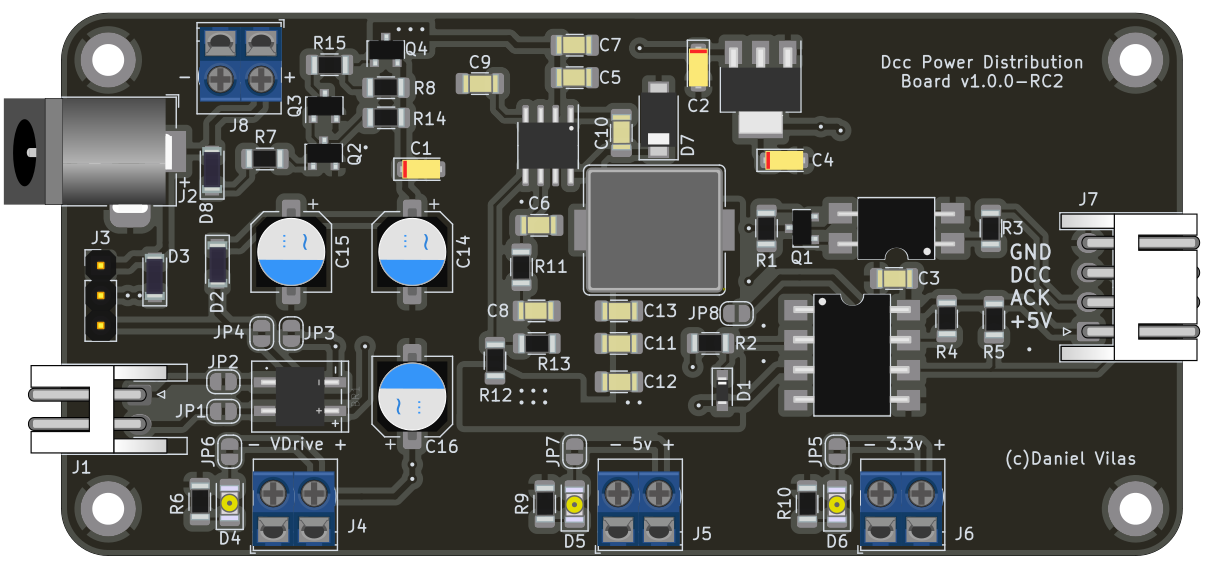
\includegraphics[scale=2]{images/front.png}};
        \end{scope}
        
        \draw [color=red](-6.2,2.4) rectangle + (2.3,-2.5); 
        \node [text width = 1.3cm] at (-5,-0.5){VDrive};
        \draw [color=red](-0.3,2.4) rectangle + (2.3,-2.5); 
        \node [text width = 1.3cm] at (1,-0.5){+5V};
        \draw [color=red](4.1,2.4) rectangle + (2.3,-2.5); 
        \node [text width = 1.3cm] at (5.4,-0.5){+3.3V};
        \draw [color= yellow, line width=2pt] (-4.45,2.05) circle[radius=0.3];
        \draw [color= yellow, line width=2pt] (-5.95,2.05) circle[radius=0.3];
        \draw [color= yellow, line width=2pt] (0.2,2.05) circle[radius=0.3];
        \draw [color= yellow, line width=2pt] (1.1,2.05) circle[radius=0.3];
        \draw [color= yellow, line width=2pt] (4.5,2.05) circle[radius=0.3];
        \draw [color= yellow, line width=2pt] (5.65,2.05) circle[radius=0.3];
    \end{tikzpicture}
    \caption{Salida Voltaje y Corriente}
    \label{fig:VccOutConnectors2}
\end{figure}
